%Yuga_counter_example_delete.tex


\begin{figure}[c]{0.5\textwidth}
 %   \centering
    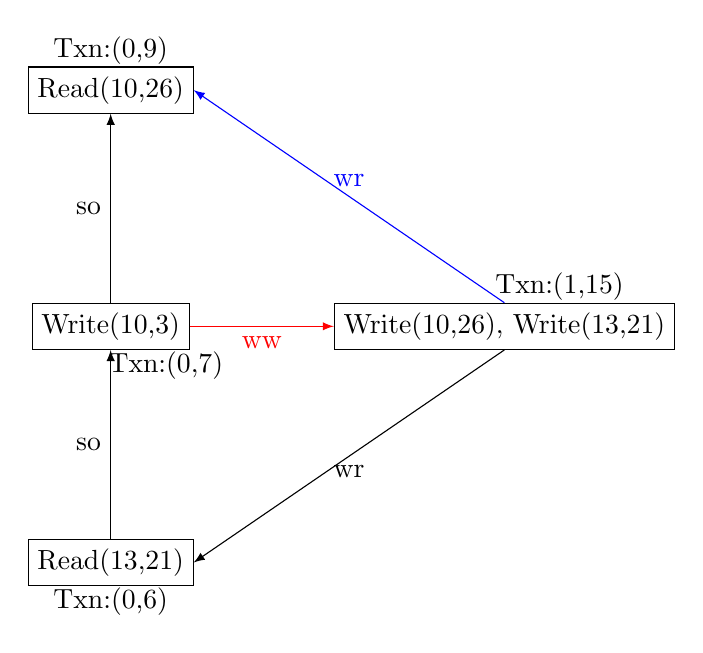
\begin{tikzpicture}[model/.style = {draw, minimum size = 15pt},  node distance = 0.5cm and 1.5cm]
        \node[model] (07) at (0,0) {Write(10,3)};
        \node (textof07) at (0.7,-0.5) {Txn:(0,7)};
        \node[model] (06) at (0,-3) {Read(13,21)};
        \node (textof06) at (0,-3.5) {Txn:(0,6)};
        \node[model] (115) at (5,0) {Write(10,26), Write(13,21)};
        \node (textof115) at (5.7,0.5) {Txn:(1,15)};
        \node[model] (09) at (0,3) {Read(10,26)};
        \node (textof09) at (0,3.5) {Txn:(0,9)};
        
        \path[-latex, color=red] (07.east) edge node[below] {ww} (115.west); 
        \path[-latex] (06.north) edge node[left] {so} (07.south); 
        \path[-latex] (115.south) edge node[below] {wr} (06.east); 
        \path[-latex] (07.north) edge node[left] {so} (09.south); 
        \path[-latex,color=blue] (115.north) edge node[above] {wr} (09.east); 
    \end{tikzpicture}
    \caption{Delete uncertainty.}
    \label{fig:delete-yuga}
\end{figure}